% Standalone architecture figure. Compile: pdflatex architecture.tex
% main.tex includes the resulting architecture.pdf with \includegraphics.
\documentclass[tikz,border=6pt]{standalone}
\usepackage{times}
\usepackage{amsmath,amssymb}
\usetikzlibrary{positioning,arrows.meta,calc,fit}
\DeclareMathOperator{\trace}{tr}
\DeclareMathOperator{\Cov}{Cov}
\begin{document}
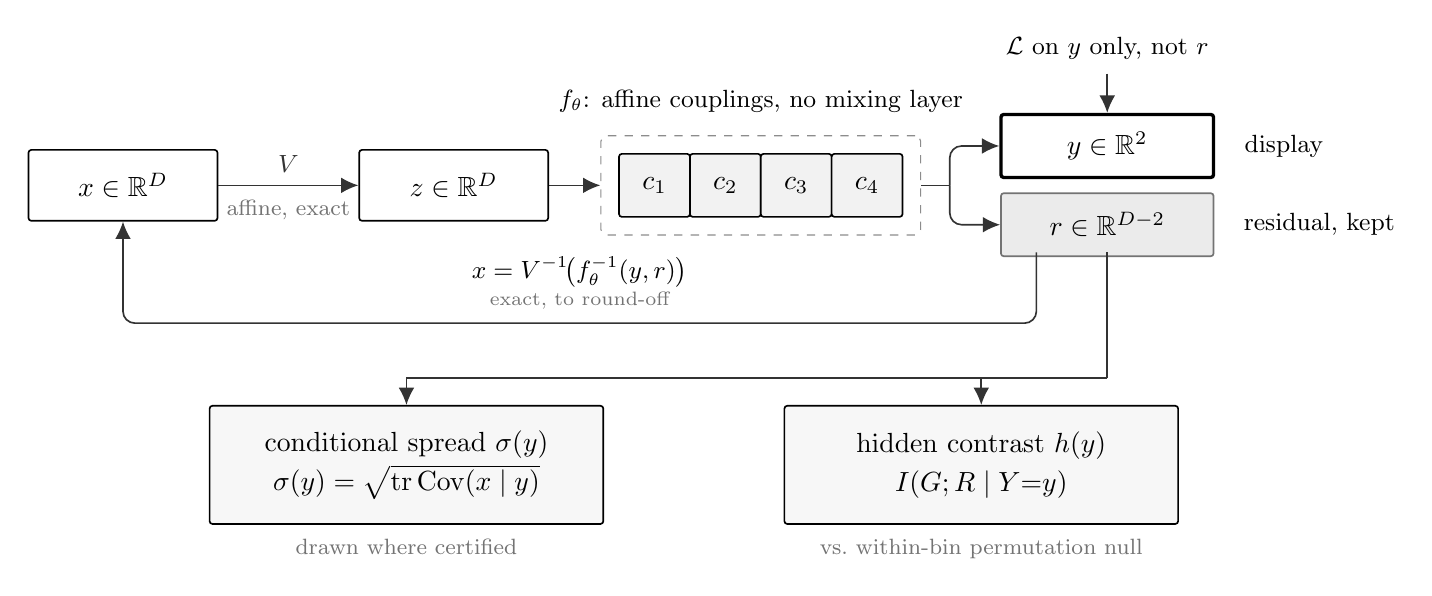
\begin{tikzpicture}[
  font=\normalsize,
  box/.style   = {draw=black, semithick, rounded corners=1pt, fill=white, align=center,
                  inner sep=1.6mm, minimum height=9mm, minimum width=24mm},
  cbox/.style  = {box, minimum width=9mm, minimum height=8mm, fill=black!5},
  obox/.style  = {box, minimum width=27mm, minimum height=8mm},
  res/.style   = {obox, draw=black!55, fill=black!8},
  disp/.style  = {box, fill=black!3, minimum width=50mm, minimum height=15mm},
  tag/.style   = {font=\small},
  sub/.style   = {font=\footnotesize, text=black!55, align=center},
  arr/.style   = {-{Latex[length=2.2mm,width=2mm]}, semithick, black!80},
  line/.style  = {semithick, black!80}]

% pipeline row (y = 0)
\node[box] (x) at (0,0)   {$x \in \mathbb{R}^{D}$};
\node[box] (z) at (4.2,0) {$z \in \mathbb{R}^{D}$};

\foreach \i/\p in {1/6.75, 2/7.65, 3/8.55, 4/9.45}
  \node[cbox] (c\i) at (\p,0) {$c_{\i}$};
\node[draw=black!45, dashed, rounded corners=2pt, inner sep=2.2mm,
      fit=(c1)(c4)] (cgrp) {};

\node[obox, very thick] (y) at (12.5, 0.50) {$y \in \mathbb{R}^{2}$};
\node[res]              (r) at (12.5,-0.50) {$r \in \mathbb{R}^{D-2}$};

\draw[arr] (x) -- node[tag, midway, above=0.4mm] {$V$}
                  node[sub, midway, below=0.6mm] {affine, exact} (z);
\draw[arr] (z) -- (cgrp);

% fan-out from the coupling stack into the two output blocks
\coordinate (split) at (10.50,0);
\draw[line] (cgrp.east) -- (split);
\draw[arr, rounded corners=1.5mm] (split) |- (y.west);
\draw[arr, rounded corners=1.5mm] (split) |- (r.west);

\node[tag, above=1.6mm of cgrp] {$f_\theta$: affine couplings, no mixing layer};
\node[tag, anchor=west] at ($(y.east)+(2.5mm,0)$) {display};

% the layout loss is applied to the display coordinates alone; r is left free
\draw[arr] (12.50,1.42) -- (y.north);
\node[tag, anchor=south] at (12.50,1.48) {$\mathcal{L}$ on $y$ only, not $r$};
\node[tag, anchor=west] at ($(r.east)+(2.5mm,0)$) {residual, kept};

% exact inverse (return path)
\draw[arr, rounded corners=1.5mm]
  (11.60,-0.85) -- (11.60,-1.75) -- (0,-1.75) -- (x.south);
\node[tag, anchor=south, align=center] at (5.80,-1.70)
  {$x = V^{-1}\!\big(f_\theta^{-1}(y,r)\big)$\\[-0.4mm]
   {\scriptsize\color{black!55}exact, to round-off}};

% displays row: two certified displays taken from the one fit, the spread field and
% the hidden-contrast field
\draw[line] (12.50,-0.85) -- (12.50,-2.45);
\draw[line] (12.50,-2.45) -- (3.60,-2.45);

\node[disp] (d1) at (3.60,-3.55)
  {conditional spread $\sigma(y)$\\[0.8mm]
   $\sigma(y)=\sqrt{\trace\Cov(x \mid y)}$};
\node[disp] (d2) at (10.90,-3.55)
  {hidden contrast $h(y)$\\[0.8mm]
   $I(G;R \mid Y{=}y)$};

\foreach \n in {d1,d2} \draw[arr] (\n.north |- 0,-2.45) -- (\n.north);

% each display carries its own certificate and is drawn only where it passes;
% the contrast field is calibrated against a within-screen-bin permutation null
\node[sub, anchor=north] at ($(d1.south)+(0,-0.6mm)$)
  {drawn where certified};
\node[sub, anchor=north] at ($(d2.south)+(0,-0.6mm)$)
  {vs.\ within-bin permutation null};

\end{tikzpicture}
\end{document}
